\UseRawInputEncoding
\documentclass[a4paper, 14pt]{extarticle}

% Поля
%--------------------------------------
\usepackage{geometry}
\geometry{a4paper,tmargin=2cm,bmargin=2cm,lmargin=3cm,rmargin=1cm}
%--------------------------------------


%Russian-specific packages
%--------------------------------------
\usepackage[T2A]{fontenc}
\usepackage[utf8]{inputenc} 
\usepackage[english, main=russian]{babel}
\usepackage{cmap}
%--------------------------------------

\usepackage{textcomp}

% Красная строка
%--------------------------------------
\usepackage{indentfirst}               
%--------------------------------------             


%Graphics
%--------------------------------------
\usepackage{graphicx}
\graphicspath{ {./images/} }
\usepackage{wrapfig}
%--------------------------------------

% Полуторный интервал
%--------------------------------------
\linespread{1.3}                    
%--------------------------------------

%Выравнивание и переносы
%--------------------------------------
% Избавляемся от переполнений
\sloppy
% Запрещаем разрыв страницы после первой строки абзаца
\clubpenalty=10000
% Запрещаем разрыв страницы после последней строки абзаца
\widowpenalty=10000
%--------------------------------------

%Списки
\usepackage{enumitem}

%Подписи
\usepackage{caption} 

%Гиперссылки
\usepackage{hyperref}

\hypersetup {
	unicode=true
}

%Рисунки
%--------------------------------------
\DeclareCaptionLabelSeparator*{emdash}{~--- }
\captionsetup[figure]{labelsep=emdash,font=onehalfspacing,position=bottom}
%--------------------------------------

\usepackage{tempora}
\usepackage{amsmath}
\usepackage[dvipsnames]{xcolor}
\usepackage{listings}
\lstset{
  belowcaptionskip=1\baselineskip,
  breaklines=true,
  frame=L,
  xleftmargin=\parindent,
  language=Java,
  showstringspaces=false,
  basicstyle=\footnotesize\ttfamily,
  keywordstyle=\bfseries\color{blue},
  commentstyle=\itshape\color{purple},
  identifierstyle=\color{black},
  stringstyle=\color{red},
  numbers=left,           
  numberstyle=\tiny\color{gray}, 
  numbersep=10pt,      
  % ------------------------------
}

%--------------------------------------
%			НАЧАЛО ДОКУМЕНТА
%--------------------------------------

\begin{document}

%--------------------------------------
%			ТИТУЛЬНЫЙ ЛИСТ
%--------------------------------------
\begin{titlepage}
\thispagestyle{empty}
\newpage


%Шапка титульного листа
%--------------------------------------
\vspace*{-60pt}
\hspace{-65pt}
\begin{minipage}{0.3\textwidth}
\hspace*{-20pt}\centering

\includegraphics[width=\textwidth]{emblem}
\end{minipage}
\begin{minipage}{0.67\textwidth}\small \textbf{
\vspace*{-0.7ex}
\hspace*{-6pt}\centerline{Министерство науки и высшего образования Российской Федерации}
\vspace*{-0.7ex}
\centerline{Федеральное государственное бюджетное образовательное учреждение }
\vspace*{-0.7ex}
\centerline{высшего образования}
\vspace*{-0.7ex}
\centerline{<<Московский государственный технический университет}
\vspace*{-0.7ex}
\centerline{имени Н.Э. Баумана}
\vspace*{-0.7ex}
\centerline{(национальный исследовательский университет)>>}
\vspace*{-0.7ex}
\centerline{(МГТУ им. Н.Э. Баумана)}}
\end{minipage}
%--------------------------------------

%Полосы
%--------------------------------------
\vspace{-25pt}
\hspace{-35pt}\rule{\textwidth}{2.3pt}

\vspace*{-20.3pt}
\hspace{-35pt}\rule{\textwidth}{0.4pt}
%--------------------------------------

\vspace{1.5ex}
\hspace{-35pt} \noindent \small ФАКУЛЬТЕТ\hspace{80pt} <<Информатика и системы управления>>

\vspace*{-16pt}
\hspace{47pt}\rule{0.83\textwidth}{0.4pt}

\vspace{0.5ex}
\hspace{-35pt} \noindent \small КАФЕДРА\hspace{50pt} <<Теоретическая информатика и компьютерные технологии>>

\vspace*{-16pt}
\hspace{30pt}\rule{0.866\textwidth}{0.4pt}
  
\vspace{11em}

\begin{center}
\Large {\bf Лабораторная работа № 7} \\ 
\large {\bf по курсу <<Языки и методы программирования>>} \\ 
\large <<GUI сабскрайбер и ридер MQTT>>
\end{center}\normalsize

\vspace{8em}


\begin{flushright}
  {Студент группы ИУ9-21Б Воронков А. С.\hspace*{15pt} \\
  \vspace{2ex}
  Преподаватель Посевин Д. П.\hspace*{15pt}}
\end{flushright}

\bigskip

\vfill
 

\begin{center}
\textsl{Москва 2026}
\end{center}
\end{titlepage}
%--------------------------------------
%		КОНЕЦ ТИТУЛЬНОГО ЛИСТА
%--------------------------------------

\renewcommand{\ttdefault}{pcr}

\setlength{\tabcolsep}{3pt}
\newpage
\setcounter{page}{2}

\section{Цель}\label{Sect::task}
\par 
Целью лабораторной работы является приобретение навыка разработки на языке 
JAVA приложения выполняющего запись данных в топик публичного MQTT брокера и 
приложения чтения данных из топика. 
\section{Задание}
\begin{enumerate}
    \item Реализовать простой чатик
    \item Реализовать приложение для подсчета евклидовой нормы вектора
\end{enumerate}
\pagebreak
\section{Практическая реализация}
Проект lab7: код файла Publisher.java
\begin{lstlisting}
    import org.eclipse.paho.client.mqttv3.*;
import java.util.Scanner;


public class Publisher {
    private MqttClient client;
    private String topic = "IU/9/voronkov";

    public Publisher() throws MqttException {
        String broker = "tcp://broker.emqx.io:1883";
        //String broker = "tcp://192.168.43.204:1883";
        //String broker = "tcp://localhost:1883";
        String clientId = "voronkov_publisher";
        client = new MqttClient(broker, clientId);
        client.connect();
    }
        public void sendMessage(String text) {
            try{
                client.publish(topic, new MqttMessage(text.getBytes()));
            } catch (MqttException e) {
                e.printStackTrace();
            }
        }
    }
\end{lstlisting}
\per
Проект lab7: код файла Subscriber.java
\begin{lstlisting}
    import org.eclipse.paho.client.mqttv3.*;
import javax.swing.*;


public class Subscriber {
    private MqttClient client;
    private String topic = "IU/9/voronkov";
    private PictureForm1 gui;

    public Subscriber(PictureForm1 gui  ) throws MqttException{
        String broker = "tcp://broker.emqx.io:1883";
        //String broker = "tcp://192.168.43.204:1883";
        //String broker = "tcp://localhost:1883";
        String clientId = "voronkov_subscriber";
        try {
            this.client = new MqttClient(broker, clientId);
            MqttConnectOptions opts = new MqttConnectOptions();

            client.setCallback(new MqttCallback() {
                public void messageArrived(String topic, MqttMessage message) throws Exception {
                    String mes = new String(message.getPayload());
                    System.out.println("message content: " + mes);
                    try {
                        SwingUtilities.invokeLater(() -> {
                            gui.updateLog(mes);
                        });

                    } catch (NumberFormatException e) {
                        System.out.println("Incorrect input");
                    }
                }

                public void connectionLost(Throwable cause) {
                    System.out.println("connectionLost: " + cause.getMessage());
                }

                public void deliveryComplete(IMqttDeliveryToken token) {
                    System.out.println("deliveryComplete: " + token.isComplete());
                }
            });

            System.out.println("Connecting to broker...");
            client.connect(opts);

            client.subscribe(topic);
            System.out.println("waiting");
        } catch (MqttException e) {
            System.err.println("Ошибка MQTT: " + e.getMessage());
            e.printStackTrace();
        }
    }
}
\end{lstlisting}
\par
Проект lab7: код файла Subscriber.java
\begin{lstlisting}
    import org.eclipse.paho.client.mqttv3.MqttException;

import javax.swing.*;
import java.awt.event.*;
import java.time.LocalDate;
import java.time.format.DateTimeFormatter;
import java.time.LocalTime;

public class PictureForm1 {
    private JPanel mainPanel;
    private JSpinner xSpinner;
    private JSpinner ySpinner;
    private JSpinner zSpinner;
    private JTextArea textArea;
    private JTextPane textPane1;
    private JButton sendButton;
    private JTextField textField1;
    private JTextField textField2;
    private JButton deleteChatButton;
    private JTextArea textArea1;
    private Publisher publisher;
    private String username = "Тёма";
    public void updateLog(String text) {
        if (text.equals("delete")) {
            textArea.setText("");
        } else {
            textArea.append(gtTime() + " " + text + "\n");
            textArea.setCaretPosition(textArea.getDocument().getLength());
        }
    }

    public String gtTime() {
        LocalDate date = LocalDate.now();
        String formatted = date.format(DateTimeFormatter.ofPattern("dd.MM.yyyy"));

        LocalTime time = LocalTime.now();
        String formattedTime = time.format(DateTimeFormatter.ofPattern("HH:mm"));
        return formatted + " " + formattedTime;
    }


    public PictureForm1(Publisher publisher) {
        this.publisher = publisher;


        textField1.addActionListener(new ActionListener() {
            @Override
            public void actionPerformed(ActionEvent e) {
                username = textField2.getText();
                String text = textField1.getText();
                if (!text.isEmpty()) {
                    publisher.sendMessage(username + ": " + text);
                    textField1.setText("");
                }
            }
        });
        sendButton.addActionListener(new ActionListener() {
            @Override
            public void actionPerformed(ActionEvent e) {
                username = textField2.getText();
                publisher.sendMessage(textField1.getText());
                textField1.setText("");
            }
        });
        textField2.setText(username);
        deleteChatButton.addActionListener(new ActionListener() {
            @Override
            public void actionPerformed(ActionEvent e) {
                publisher.sendMessage("delete");
            }
        });
    }


    public static void main(String[] args) {
        try {
            Publisher pub = new Publisher();
            PictureForm1 form = new PictureForm1(pub);
            JFrame frame = new JFrame("Чат");
            frame.setContentPane(form.mainPanel);
            frame.setDefaultCloseOperation(JFrame.EXIT_ON_CLOSE);
            frame.pack();
            frame.setLocationRelativeTo(null);
            frame.setVisible(true);
            form.textField1.requestFocusInWindow();
            new Subscriber(form);
        } catch (MqttException e) {
            e.printStackTrace();
        }
    }
}
\end{lstlisting}
\par
Проект rtfm7: код файла Publisher.java
\begin{lstlisting}
import org.eclipse.paho.client.mqttv3.*;
import java.util.Scanner;


public class Publisher {
    private MqttClient client;
    private String topic = "IU/9/voronkov";

    public Publisher() throws MqttException {
        String broker = "tcp://broker.emqx.io:1883";
        String clientId = "voronkov_publisher";
        client = new MqttClient(broker, clientId);
        client.connect();
    }
        public void sendMessage(String text) {
            try{
                client.publish(topic, new MqttMessage(text.getBytes()));
            } catch (MqttException e) {
                e.printStackTrace();
            }
        }
    }
\end{lstlisting}
\par
Проект rtfm7: код файла Subscriber.java
\begin{lstlisting}
import org.eclipse.paho.client.mqttv3.*;
import javax.swing.*;


public class Subscriber {
    private MqttClient client;
    private String topic = "IU/9/voronkov";
    private PictureForm1 gui;

    public Subscriber(PictureForm1 gui  ) throws MqttException{
        String broker = "tcp://broker.emqx.io:1883";
        String clientId = "voronkov_subscriber";
        try {
            this.client = new MqttClient(broker, clientId);
            MqttConnectOptions opts = new MqttConnectOptions();

            client.setCallback(new MqttCallback() {
                public void messageArrived(String topic, MqttMessage message) throws Exception {
                    String mes = new String(message.getPayload());
                    System.out.println("message content: " + mes);
                    String[] nums = mes.split(" ");
                    if (nums.length != 3) {
                        System.out.println("Incorrect input");
                        return;
                    }
                    try {
                        Vector vc = new Vector(mes);
                        double n = vc.norm();
                        System.out.println("Euclidian norm: " + n);
                        String result = "Вектор: " + mes + " | Норма: " + n;
                        SwingUtilities.invokeLater(() -> {
                            gui.updateLog(result);
                        });

                    } catch (NumberFormatException e) {
                        System.out.println("Incorrect input");
                    }
                }

                public void connectionLost(Throwable cause) {
                    System.out.println("connectionLost: " + cause.getMessage());
                }

                public void deliveryComplete(IMqttDeliveryToken token) {
                    System.out.println("deliveryComplete: " + token.isComplete());
                }
            });

            System.out.println("Connecting to broker...");
            client.connect(opts);

            client.subscribe(topic);
            System.out.println("waiting");
        } catch (MqttException e) {
            System.err.println("Ошибка MQTT: " + e.getMessage());
            e.printStackTrace();
        }
    }
}
\end{lstlisting}
\par
Проект rtfm7: код файла Vector.java
\begin{lstlisting}
    import java.lang.Math;

public class Vector {
    double x, y, z;
    public Vector (double x, double y, double z) {
        this.x = x;
        this.y = y;
        this.z = z;
    }

    public Vector (String s) {
        String[] nums = s.split(" ");
        double x, y, z;
        this.x = Double.parseDouble(nums[0]);
        this.y = Double.parseDouble(nums[1]);
        this.z = Double.parseDouble(nums[2]);
    }

    public void changeX(double x) { this.x = x;}
    public void changeY(double y) { this.y = y;}
    public void changeZ(double z) { this.z = z;}


    public double norm() {
        return Math.sqrt(x*x + y*y + z*z);
    }

    public String toString() {
        return x + " " + y + " " + z;
    }
}
\end{lstlisting}
\par
Проект rtfm7: код файла PictureForm1.java
\begin{lstlisting}
import org.eclipse.paho.client.mqttv3.MqttException;

import javax.swing.*;
import javax.swing.event.ChangeEvent;
import javax.swing.event.ChangeListener;

public class PictureForm1 {
    private JPanel mainPanel;
    private JSpinner xSpinner;
    private JSpinner ySpinner;
    private JSpinner zSpinner;
    private JTextArea textArea;
    private Publisher publisher;
    public void updateLog(String text) {
        textArea.append(text + "\n");
        textArea.setCaretPosition(textArea.getDocument().getLength());
    }

    public PictureForm1(Publisher publisher) {
        this.publisher = publisher;
        xSpinner.setValue(10);
        ySpinner.setValue(10);
        zSpinner.setValue(10);
        Vector vector = new Vector(10, 10, 10);
        xSpinner.addChangeListener(new ChangeListener() {
            @Override
            public void stateChanged(ChangeEvent e) {
                int x = (int)xSpinner.getValue();
                vector.changeX(x);
                publisher.sendMessage(vector.toString());
            }
        });
        ySpinner.addChangeListener(new ChangeListener() {
            @Override
            public void stateChanged(ChangeEvent e) {
                int y = (int)ySpinner.getValue();
                vector.changeY(y);
                publisher.sendMessage(vector.toString());
            }
        });
        zSpinner.addChangeListener(new ChangeListener() {
            @Override
            public void stateChanged(ChangeEvent e) {
                int z = (int)zSpinner.getValue();
                vector.changeZ(z);
                publisher.sendMessage(vector.toString());
            }
        });

    }


    public static void main(String[] args) {
        try {
            Publisher pub = new Publisher();
            PictureForm1 form = new PictureForm1(pub);
            JFrame frame = new JFrame("Вектор");
            frame.setContentPane(form.mainPanel);
            frame.setDefaultCloseOperation(JFrame.EXIT_ON_CLOSE);
            frame.pack();
            frame.setLocationRelativeTo(null);
            frame.setVisible(true);
            new Subscriber(form);
        } catch (MqttException e) {
            e.printStackTrace();
        }
    }
}
\end{lstlisting}

\section{Результаты}
В результате лабораторной работы было создано два приложения. Одно представляет из себя чат для общения нескольких пользователей через один топик. Второе приложение реализует отправку координат вектора и их чтение из соответствующего топика и подсчет евклидовой нормы вектора

\begin{center}
    \nopagebreak
    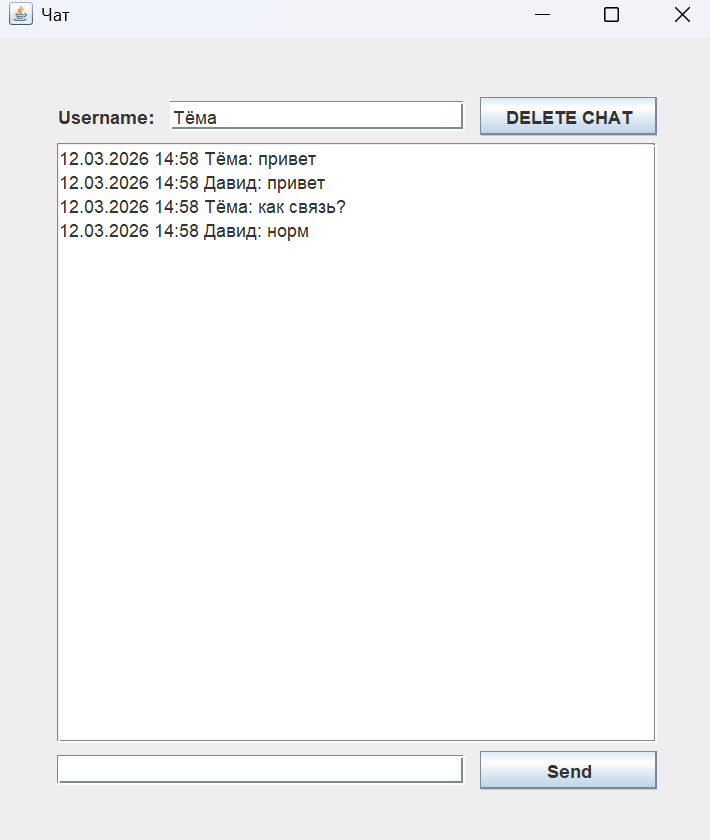
\includegraphics[width=0.85\textwidth]{lab7_1}
    \captionsetup{justification=centering}
    \captionof{figure}{Визуализация работы чатика}

    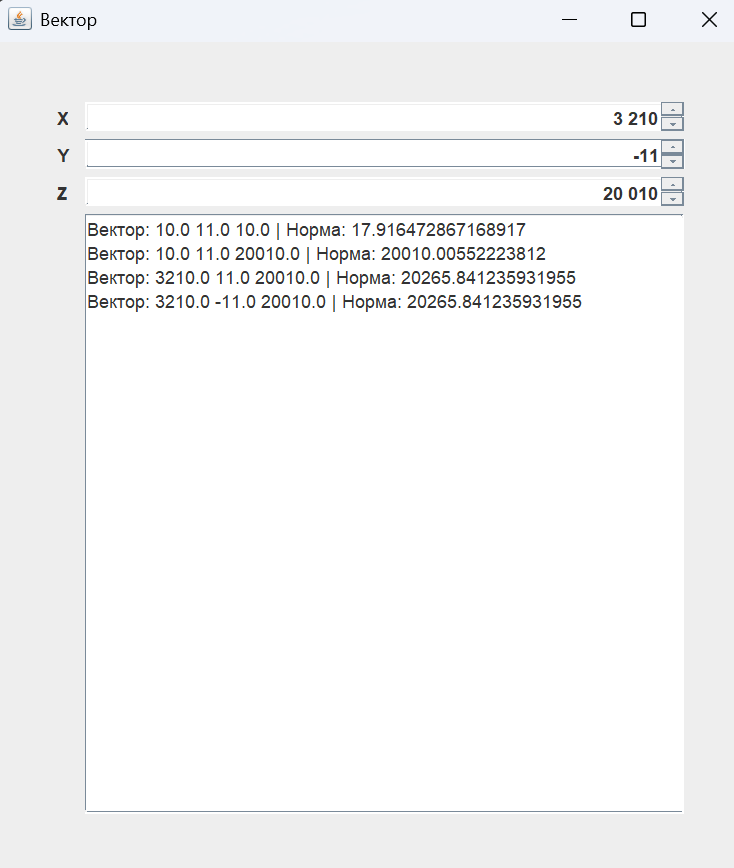
\includegraphics[width=0.85\textwidth]{lab7_2}
    \captionsetup{justification=centering}
    \captionof{figure}{Визуализация работы приложения учета векторов}
\end{center}

\section{Вывод}
В данной лабораторной работе были получены навыки работы с протоколом MQTT. Была написана своя читалка и писалка
\end{document}